\documentclass[12pt,a4paper]{article}
\usepackage{inverba}

\newcommand{\userName}{Cullyn Newman} 
\newcommand{\class}{BI 358} 
\newcommand{\institution}{Portland State University} 
\newcommand{\theTitle}{\color{g-Leaf} Discussion Questions}

\begin{document}
%%%%%%%%%%%%%%%%%%%%%%%%%%%%%%%%%%%%%%%%%%%%%%%%%%%%%%%%%%%%%%%%%%%%%
\tableofcontents
\cleardoublepage
\fancyhead{}
%%%%%%%%%%%%%%%%%%%%%%%%%%%%%%%%%%%%%%%%%%%%%%%%%%%%%%%%%%%%%%%%%%%%%

%%%%%%%%%%%%%%%%%%%%%%%%%%%%% Week 5 %%%%%%%%%%%%%%%%%%%%%%%%%%%%%
%\begingroup
\clearpage
\section*{Week 5}\phantomsection
\addcontentsline{toc}{section}{\textbf{Week 5}}
\fancyhead[R]{\hyperlink{home}{Week 5}}

\fancyhead[L]{\hyperlink{home}{Heritability Exercise}}
\subsection{Heritability Exercise}
\begin{enumerate}
    {\color{G-Moon}\item Approximately, what is the heritability of running speed in the breeder’s dog population?}
{\small\begin{lstlisting}
# data given used to create dataframe
d = {
'Midoffspring':[10.8, 8, 8, 9.7, 6.6, 6.2, 12.5, 7.4,
3.4, 6.7, 7.9, 13.6, 7.4, 12.1, 11.3], 
'Midparent':[12.7, 7.6, 14.4, 4.3, 11.3, 12.5, 8.9,
8.2, 6.3, 12.7, 13.9, 7.3, 5.9, 12.8, 12.5]
}
df = pd.DataFrame(data=d)

# get coefficients of linear fit
slope, intercept, r_value, p_value, std_err = 
stats.linregress(df['Midparent'], df['Midoffspring'])

# plot graph, make label for
ax = sns.regplot(df['Midparent'], df['Midoffspring'], 
line_kws={'label':
"y={0:.1f}x+{1:.1f}".format(slope,intercept)})

# plot legend
ax.legend()
plt.show()
\end{lstlisting}}
\begin{center}
    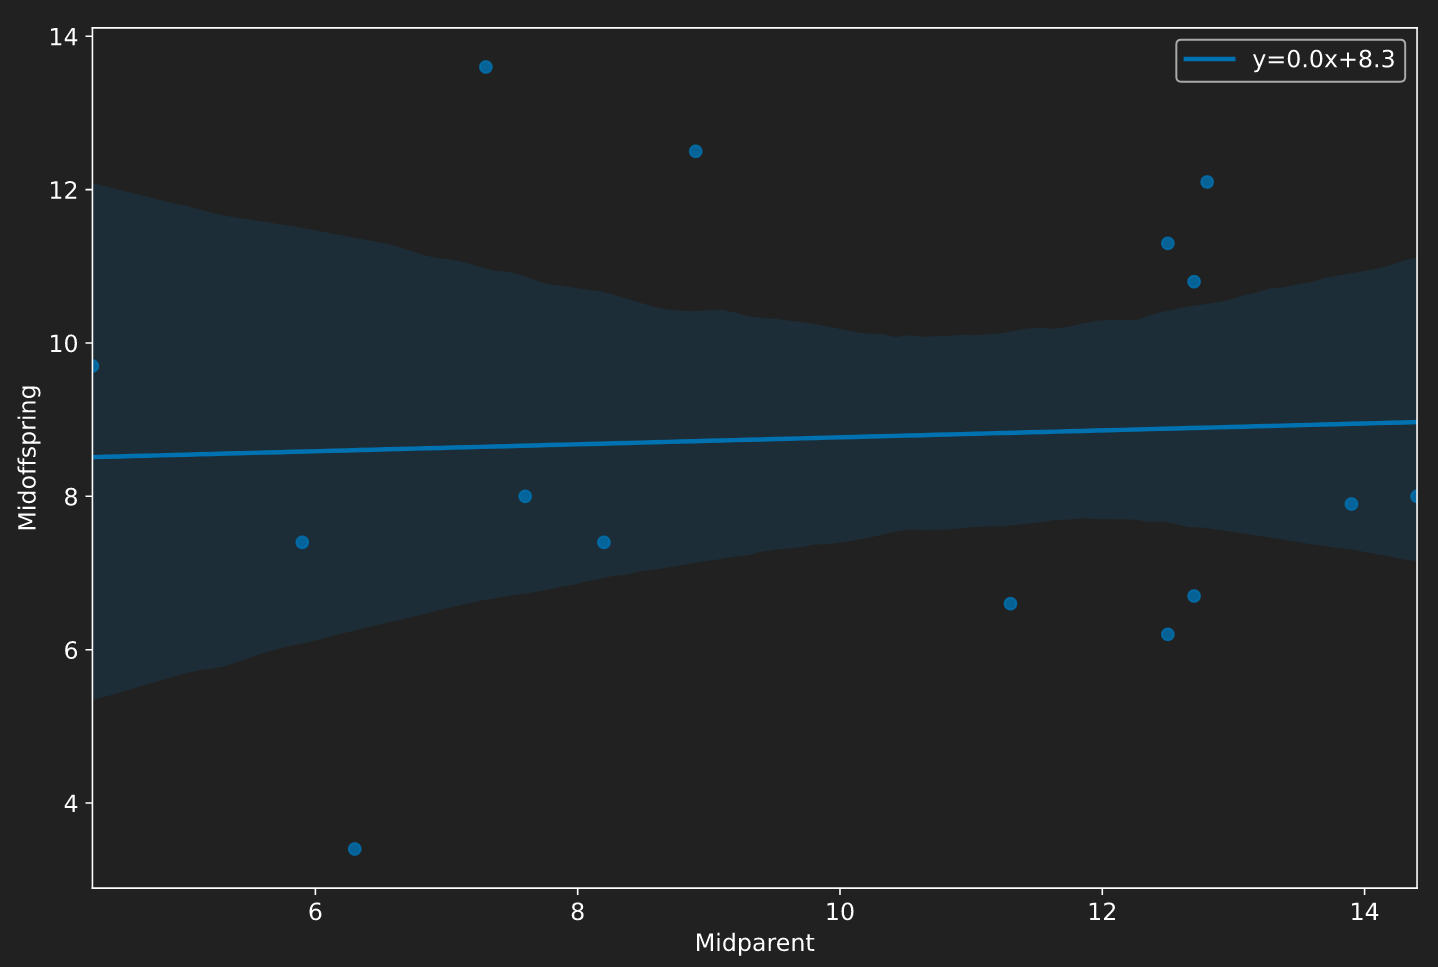
\includegraphics[scale=0.35]{images/heritability.png}
\end{center}
    {\color{G-Moon}\item If she selectively breeds her dogs, will the next generation run substantially faster than the dogs she has now?}
        \begin{itemize}
            \item No, very low heritability, nearly 0. (y=0.0x+8.3)
        \end{itemize}
    {\color{G-Moon}\item What else would you suggest the breeder try if she wants to win more races?}
        \begin{itemize}
            \item Continue to track the midoffspring and midparent speeds, selectively breeding those who tend have a higher heritability ratio in regards to speed
            \item Such a low slope could indicate low heritability of speed, so might be more useful to pursue environmental factors.
        \end{itemize}
\end{enumerate}



%\endgroup
%%%%%%%%%%%%%%%%%%%%%%%%%%%%% Week 5%%%%%%%%%%%%%%%%%%%%%%%%%%%%%





%%%%%%%%%%%%%%%%%%%%%%%%%%%%% Chapter 4 %%%%%%%%%%%%%%%%%%%%%%%%%%%%%
%\begingroup
\clearpage
\section*{Week 4}\phantomsection
\addcontentsline{toc}{section}{\textbf{Week 4}}
\fancyhead[R]{\hyperlink{home}{Week 4}}

\fancyhead[L]{\hyperlink{home}{Molecular Clock}}
\subsection{Molecular Clock}
\begin{align*}
    \textbf{CHEETA EXAMPLE:}\\
    \text{{\color{p-Lush}Divergence: 5.2\%} per 1mya, {\color{g-Fresh} Diversity for this locus: 0.182\%} per [x=time]}\\
    \frac{{\color{g-Fresh}0.182}}{x} = \frac{{\color{p-Lush}5.2\%}}{\num{1e6}}\\
    \num{1.82e5}= 5.2x\\
    x = \frac{\num{1.82e5}}{5.2} = \SI{35000}{yrs}\\ 
    \text{{\color{p-Lush}Divergence: 6.5\%} per 1mya, {\color{g-Fresh}Diversity for this locus: 0.182\%} per [x=time]}\\
    \frac{{\color{g-Fresh}0.182}}{x} = \frac{{\color{p-Lush}6.5\%}}{\num{1e6}}\\
    \num{1.82e5}= 6.5x\\
    x = \frac{\num{1.82e5}}{6.5} = \SI{28000}{yrs}\\ 
    \textbf{DOGS EXAMPLE:}\\
    \text{{\color{p-Lush}Divergence: 7.5\%} per 1mya, {\color{g-Fresh}Diversity for this locus: 1\%} per [x=time]}\\
    {\color{G-Moon}\text{Note: 0.075, and 0.01 converted to \%}}\\
    \frac{{\color{g-Fresh}1}}{x} = \frac{{\color{p-Lush}7.5\%}}{\num{1e6}}\\
    \num{1e6}= 7.5x\\
    x = \frac{\num{1e6}}{7.5} = \SI{133333}{yrs}\\
\end{align*}

\newpage
\fancyhead[L]{\hyperlink{home}{Zika Evolution}}
\subsection{Zika Evolution}
{\color{darklc} Metsky HC et al. 2017. Zika virus evolution and spread in the Americas. Nature 546: 411-415. $\mapsto$}
\subsubsection{Background}
\begin{itemize}
    {\color{G-Moon}\item What was known about Zika virus evolution before this paper was written?}
        \begin{itemize}
            \item Fewer than 100 ZIKV genomes were previously sequenced directly from clinical samples, providing little information about it's epidemiology and evolution.
            \item The virus had a link to birth defects and other neurological complications.
        \end{itemize}
    {\color{G-Moon}\item What were the goals of the authors of this paper?}
        \begin{itemize}
            \item "to gain a deeper understanding of the viral populations underpinning the ZIKV epidemic by extensive genome sequencing."
            \item Understand how sequences are changing and how selection might be acting on the virus.
            \item Where the virus originated.
        \end{itemize}
\end{itemize}

\subsubsection{Methods}
\begin{itemize}
    {\color{G-Moon}\item What taxa were sampled for this study and where specifically were they from?}
        \begin{itemize}
            \item Samples were collected from United States, Guatemala/ El Salvador, Haiti, Dominican Republic, Honduras, Puerto Rico, Martinique, Jamaica, Brazil, and Columbia.
            \item Puerto Rico, Honduras, Columbia, and the Caribbean (includes USA) were the four well supported clades.
        \end{itemize}
    {\color{G-Moon}\item Why was this sampling strategy important to address their goals?}
        \begin{itemize}
            \item Unbiased metagenomic sequencing of 38 samples proved to have insufficient ZIKV RNA for genome assembly, so PCR amplification (110/229 genomes) and hybrid capture (37/66 genomes) had to be used for enrichment.
            \item They had a short sampling period, so deleterious mutations were hard to catch, as well as other changes. They needed a large and diverse set of samples to establish a molecular clock and a substitution rate.
        \end{itemize}
    {\color{G-Moon}\item How was evidence of selection on the Zika virus genome determined?}
        \begin{itemize}
            \item Total of 110 genomes, plus 64 previous published genomes were used in a reconstrued phylogenetic tree based on a molecular clock. 
            \item Each lineage was then traced back to root and used to estimate the substitution rate, which would provide evidence of selection.
            \item Aimed to compare ratio between synonomys and nonsynonymous mutations.
        \end{itemize}
\end{itemize}
\subsubsection{Results}
\begin{itemize}
    {\color{G-Moon}\item Looking at the results shown in Figure 2, explain how the authors arrived at the conclusion that the Zika virus outbreak originated in Brazil.}
        \begin{itemize}
            \item The Brazil ZIKV genomes appear on all deep branches of the tree, and the most recent common ancestor is the root of the tree.
        \end{itemize}
    {\color{G-Moon}\item When did the authors determine the Zika virus outbreak(s) occurred?}
        \begin{itemize}
            \item Early 2014, 95\% confidence interval from August 2013 to July 2014.
        \end{itemize}
    {\color{G-Moon}\item What was the substitution rate for the Zika virus since the outbreak in the Americas?}
        \begin{itemize}
            \item Within-outbreak substitution rate of \num{1.15e-3},  95\% confidence interval of \num{9.78e-4} to \num{1.33e-3}
            \item A 1.3--5 times higher rate than other flaviviruses.
            \item May be higher than expected as samples did not have time for purifying selection produce an effect.
        \end{itemize}
    {\color{G-Moon}\item Why did the authors search for whether there was an excess of nonsynonymous mutations in the Zika virus envelope glycoprotein (nicknamed E)?}
        \begin{itemize}
            \item "Viral surface glycoproteins are known targets for positive selection; mutations in these proteins can confer adaption to new vectors or aid immune escape."
            \item If there was an increased substitution rate it would indicate for selection.
        \end{itemize}
    {\color{G-Moon}\item Was evidence of selection found anywhere in the Zika virus genome? Explain.}
        \begin{itemize}
            \item Adaptive mutations are more likely to be found at high frequency among the nonsynonymous mutations.
            \item Strong evidence for unrestrained diversifying selection was not found due to similar nonsynonymous substitution rates compared to other coding regions.
            \item So no, no strong evidence for selection was found.
        \end{itemize}
\end{itemize}
%\endgroup
%%%%%%%%%%%%%%%%%%%%%%%%%%%%% Chapter 4 %%%%%%%%%%%%%%%%%%%%%%%%%%%%%


%%%%%%%%%%%%%%%%%%%%%%%%%%%%% Week 3 %%%%%%%%%%%%%%%%%%%%%%%%%%%%%
%\begingroup
\clearpage
\section*{Week 3}\phantomsection
\addcontentsline{toc}{section}{\textbf{Week 3}}
\fancyhead[R]{\hyperlink{home}{Week 3}}

\fancyhead[L]{\hyperlink{home}{\textit{Populus} Stimulations}}
\subsection{\textit{Populus} Stimulations}
\begin{enumerate}
    \subsubsection*{Exercise 1: Stimulating Strong Selection}
    {\color{darklc}\item  Describe how the frequency of the \textit{A} allele changes due to strong selection.}
        \begin{itemize}
            \item The frequency of the \textit{A} allele {\color{pos}increases rapidly} due to strong selection.
        \end{itemize}
    {\color{darklc}\item How many generations passed before the \textit{A} allele was fixed or lost?}
        \begin{itemize}
            \item Roughly {\color{o-Sun}60--70} generations.
        \end{itemize}
    {\color{darklc}\item How many generations passed before the \textit{a} allele was fixed or lost.}
        \begin{itemize}
            \item Roughly {\color{o-Sun}60--70} generations.
        \end{itemize}
    \subsubsection*{Exercise 2: Simulating Modereate Selection}
    {\color{darklc}\item Describe how the frequency of the \textit{A} allele changes due to slightly weaker selection.}
        \begin{itemize}
            \item Moderate sigmodal increases in frequency.
        \end{itemize}
    {\color{darklc}\item How many generations passed before the \textit{A} allele was fixed or lost?}
        \begin{itemize}
            \item Roughly {\color{o-Sun}120--130} generations.
        \end{itemize}
    {\color{darklc}\item How many generations passed before the \textit{a} allele was fixed or lost?}
        \begin{itemize}
            \item Roughly {\color{o-Sun}120--130} generations.
        \end{itemize}
    \subsubsection*{Exercise 3: Simulating Weak Selection}
    {\color{darklc}\item Describe how the frequency of the \textit{A} allele changes due to weak selection.}
        \begin{itemize}
            \item {\color{pos}Slightly increasing} exponential curve. 
        \end{itemize}
    {\color{darklc}\item How many generations passed before the \textit{A} allele was fixed or lost?}
        \begin{itemize}
            \item Was not fixed or lost after 1000 generations.
        \end{itemize}
    {\color{darklc}\item How many generations passed before the \textit{a} allele was fixed or lost?}
        \begin{itemize}
            \item Same, neither allele was not fixed or lost.
        \end{itemize}
    {\color{darklc}\item If a generation was equal to 10 years, how many years would it take for the frequency of the \textit{A} allele to double in frequency (from 10\% to 20\%)}
        \begin{itemize}
            \item About 550 generations, so approximately {\color{o-Sun}5,500} years.
        \end{itemize}
\end{enumerate}
%\endgroup
%%%%%%%%%%%%%%%%%%%%%%%%%%%%% Week 3 %%%%%%%%%%%%%%%%%%%%%%%%%%%%%

%%%%%%%%%%%%%%%%%%%%%%%%%%%%% Week 2 %%%%%%%%%%%%%%%%%%%%%%%%%%%%%
%\begingroup
\clearpage
\section*{Week 2}\phantomsection
\addcontentsline{toc}{section}{\textbf{Week 2}}
\fancyhead[R]{\hyperlink{home}{Week 2}}
\fancyhead[L]{\hyperlink{home}{Dog Domesticaion}}
\subsection{Dog Domestication}
\begin{itemize}
    \item Background and Goals
        \begin{itemize}
            {\color{darklc} \item What hypotheses about dog domestication are examined in this paper?}
                \begin{itemize}
                    \item The origin of domestic dogs was the main focus; genetic data suggests East Asia, but other data suggests Europe and Siberia. 
                \end{itemize}
            {\color{darklc} \item  What predictions do these hypotheses make? What would the expected phylogenetic trees look like under each of these hypotheses (i.e. what are the expected topologies)?}
                \begin{itemize}
                    \item The most recent common ancestor would indicate origin and genetic data would help confirm time frame.
                \end{itemize}
        \end{itemize}
    \item Methods
        \begin{itemize}
            {\color{darklc} \item  What taxa were sampled for this study?} 
                \begin{itemize}
                    \item Hypothesis was tested using DNA extracted to trace mitochondrial genomes from 18 prehistoric canids and 20 modern wolves from Eurasian and American origin. 
                \end{itemize}
            {\color{darklc} \item  What gene sequences were used for this study?}
                \begin{itemize}
                    \item Wolves, dogs, including divergent breeds, recently published chinese indigenous dogs, and coyotes. (148 mitochondrial genomes)
                \end{itemize}
            {\color{darklc} \item  What phylogenetic methods were used to reconstruct the phylogenetic tree in Figure 1?}
                \begin{itemize}
                    \item Maximum likelyhood, coalescence, and Bayesian.
                \end{itemize}
        \end{itemize}
    \item Results and Discussion
        \begin{itemize}
            {\color{darklc} \item In Figure 1, which wolf sequence is most closely related to the extant dog clade A, and what geographic region is it from?}
                \begin{itemize}
                    \item Wolves: Switzerland 2 14,500.
                    \item Dogs: Argentina, USA (8,500, 1,000) 
                \end{itemize}
            {\color{darklc} \item In Figure 1, which clade of modern dog sequences has the oldest origin? Approximately how old is this clade?}
                \begin{itemize}
                    \item Dog clade A, Russia, 18,000 years ago.
                \end{itemize}
            {\color{darklc} \item Based upon Figure 1, how many times does it appear that modern extant dogs could possibly have been domesticated?}
                \begin{itemize}
                    \item Figure 1 suggests 4, but the the authors state, {\color{G-Moon}"the inferred recent divergence of clade B from wolves now found in Sweden and Ukraine implies that is might represent a mitochondrial genome introgressed from wolves rather than one established by domestication."}
                \end{itemize}
            {\color{darklc} \item What was the topology of the phylogenetic tree that was recovered, and therefore, which hypothesis was supported?}
                \begin{itemize}
                    \item The findings support the conclusion that legacy of dogs derives from wolves of European origin.
                    \item Analysis of coalescence times support divergence time of >15,000 years ago.
                    \item Past mitochondrial and Y chromosome analysis suggestesd non-European, but had less supported data than these findings.
                \end{itemize}
        \end{itemize}
    \item Conclusions
        \begin{itemize}
            {\color{darklc} \item  What are the major conclusions of the paper?}
                \begin{itemize}
                    \item Three of four modern dog clades are more closely related to sequences from ancient European rather than extant wolves with divergence times >15,000 years ago.
                \end{itemize}
            {\color{darklc} \item  Was the taxonomic sampling sufficient to rule out alternative hypotheses? }
                \begin{itemize}
                    \item Ancient panel did not contain specimens from Middle East or China. No, no ancient dog remains older than 13,000 years are known from those regions.
                    \item The mtDNA sequence tree is well supported, but represents a single genetic locus. Independent loci could offer more power to resolve phylogenetic relations.
                \end{itemize}
        \end{itemize}
\end{itemize}

\clearpage
\fancyhead[L]{\hyperlink{home}{Changes in Speech}}
\subsection{How Farming Reshaped Our Smiles and Our Speech}
\begin{itemize}
    \item Gibbons A 2019; doi: 10.1126/science.363.6432.113
\end{itemize}
\begin{enumerate}
    {\color{darklc}\item What is this news article about?}
        \begin{itemize}
            \item How farming may have reshaped our jaws and thus indirectly influencing how we speak.
        \end{itemize}
    {\color{darklc}\item How could diet change the structure of the jaw?}
        \begin{itemize}
            \item Less wear and tear changed how jaws and teeth developped, creating an overbite with the now less worn down teeth.
        \end{itemize}
    {\color{darklc}\item How could jaw structure change speech patterns of humans?}
        \begin{itemize}
            \item Jaw and teeth placement changes how easy it is to make certain sounds, and overbites made "f" and "v" easier to make.
        \end{itemize}
    {\color{darklc}\item Are these changes in jaw structure permanent? Why or why not?}
        \begin{itemize}
            \item Not likely, if you ate diets similar to early humans your teeth would wear down more and impact from wisdom teeth would minimize overbite. Though, there may have been some lasting selection pressure for a natural overbite.
        \end{itemize}
    {\color{darklc}\item Did natural selection shape these changes in jaw structure? Explain.}
        \begin{itemize}
            \item Not likely, mostly likely from behavior change due to mostly diet change.
        \end{itemize}
    {\color{darklc}\item Can natural selection shape speech patterns? Explain.}
        \begin{itemize}
            \item Yes, sexual selection could be a significant. Or if the change in speech pattern could confer a advantage in communication.
        \end{itemize}
    {\color{darklc}\item Can you think of any parallels with other animals where diet influenced feeding structures?}
        \begin{itemize}
            \item Lots of animals, birds (finches!!), dogs, snakes. Huge impact.
        \end{itemize}
\end{enumerate}
%\endgroup
%%%%%%%%%%%%%%%%%%%%%%%%%%%%% Week 2 %%%%%%%%%%%%%%%%%%%%%%%%%%%%%
\end{document}